\section{Plug-In Components of Online Adaptation} 
\label{sec:design-space}

We frame the loop in Fig.~\ref{fig:test_time_feedback} as a \emph{harness}: a fixed online schedule with swappable components at the points where feedback is collected, transformed, and used for fine-tuning. Each round generates candidates, selects a subset for oracle evaluation, converts oracle scores into training rewards, regularizes the update, and fine-tunes the generator. As a \emph{harness}, it is finetuner-agnostic and domain-agnostic: any discrete generator with objective $\mathcal{L}_{\text{ft}}$ that consumes per-sample log-rewards and an off-policy buffer can be used; we instantiate it with DDPP-LB~\citep{rector-brooksSteeringMaskedDiscrete2024} and VIDD~\citep{suIterativeDistillationRewardGuided2025}.

We organize the components by their role in the feedback loop. \emph{Steering strategies} affect which candidates receive oracle evaluations (Sec.~\ref{sec:design-explore}); \emph{adaptation strategies} determine how observed rewards shape the model update (Sec.~\ref{sec:adaptation_design}); and \emph{objective-mismatch corrections} keep optimization aligned with accumulated feedback and valid molecules as exploration shifts the sampling distribution $p_{\theta_t}$ (Sec.~\ref{sec:design-objmismatch}). For each category, we instantiate one representative choice adapted from prior work (Table~\ref{tab:methods}). The per-knob ablations in Sec.~\ref{sec:results} then test whether these choices retain distinct value when composed.

\begin{table}[h]
\centering
\small
    \begin{tabular}{@{}p{4.4cm}p{9.3cm}@{}}
\toprule
\textbf{Knob} & \textbf{Description} \\
\midrule
$+$ CVaR~\citep{santiFlowDensityControl, wang2026efficient}            & Replace $r$ with $(r - Q_\tau)_+/(1-\tau)$, $\tau{=}0.8$ \\
$+$ Density Entropy Reg.~\citep{de2025provable}  & Add $-\gamma \log p_\theta(x)$ to log-reward, $\gamma{=}1$ \\
$+$ Thompson~\citep{thompson1933likelihood, chapelle2011empirical}        & $J{=}10$ MLP ensemble; oracle top-$K$ by $s_i \sim \mathcal{N}(\mu_i, \sigma_i^2)$ \\
$+$ Replay buffer~\citep{mnih2015human}   & Fixed-capacity FIFO with priority eviction; stratified sampling \\
$+$ Invalid penalty~\citep{wangFineTuningDiscreteDiffusion2024, ueharaELEGANT2024}  & Assign $r {=} r_{\text{inv}}$ to SMILES that fail RDKit parsing \\
\bottomrule
\end{tabular}
\caption{\textbf{\emph{Harness} knobs: plug-in components evaluated in this paper.} Each knob layers on top of finetuner and is ablated independently in Section~\ref{sec:results}, then evaluated jointly in the final recipe of Sec.~\ref{sec:results-method}.}
\label{tab:methods}
\vspace{-0.2in}
\end{table}



\subsection{Steering Strategies}\label{sec:design-explore}

%\begin{figure}[b]
%  \centering
%  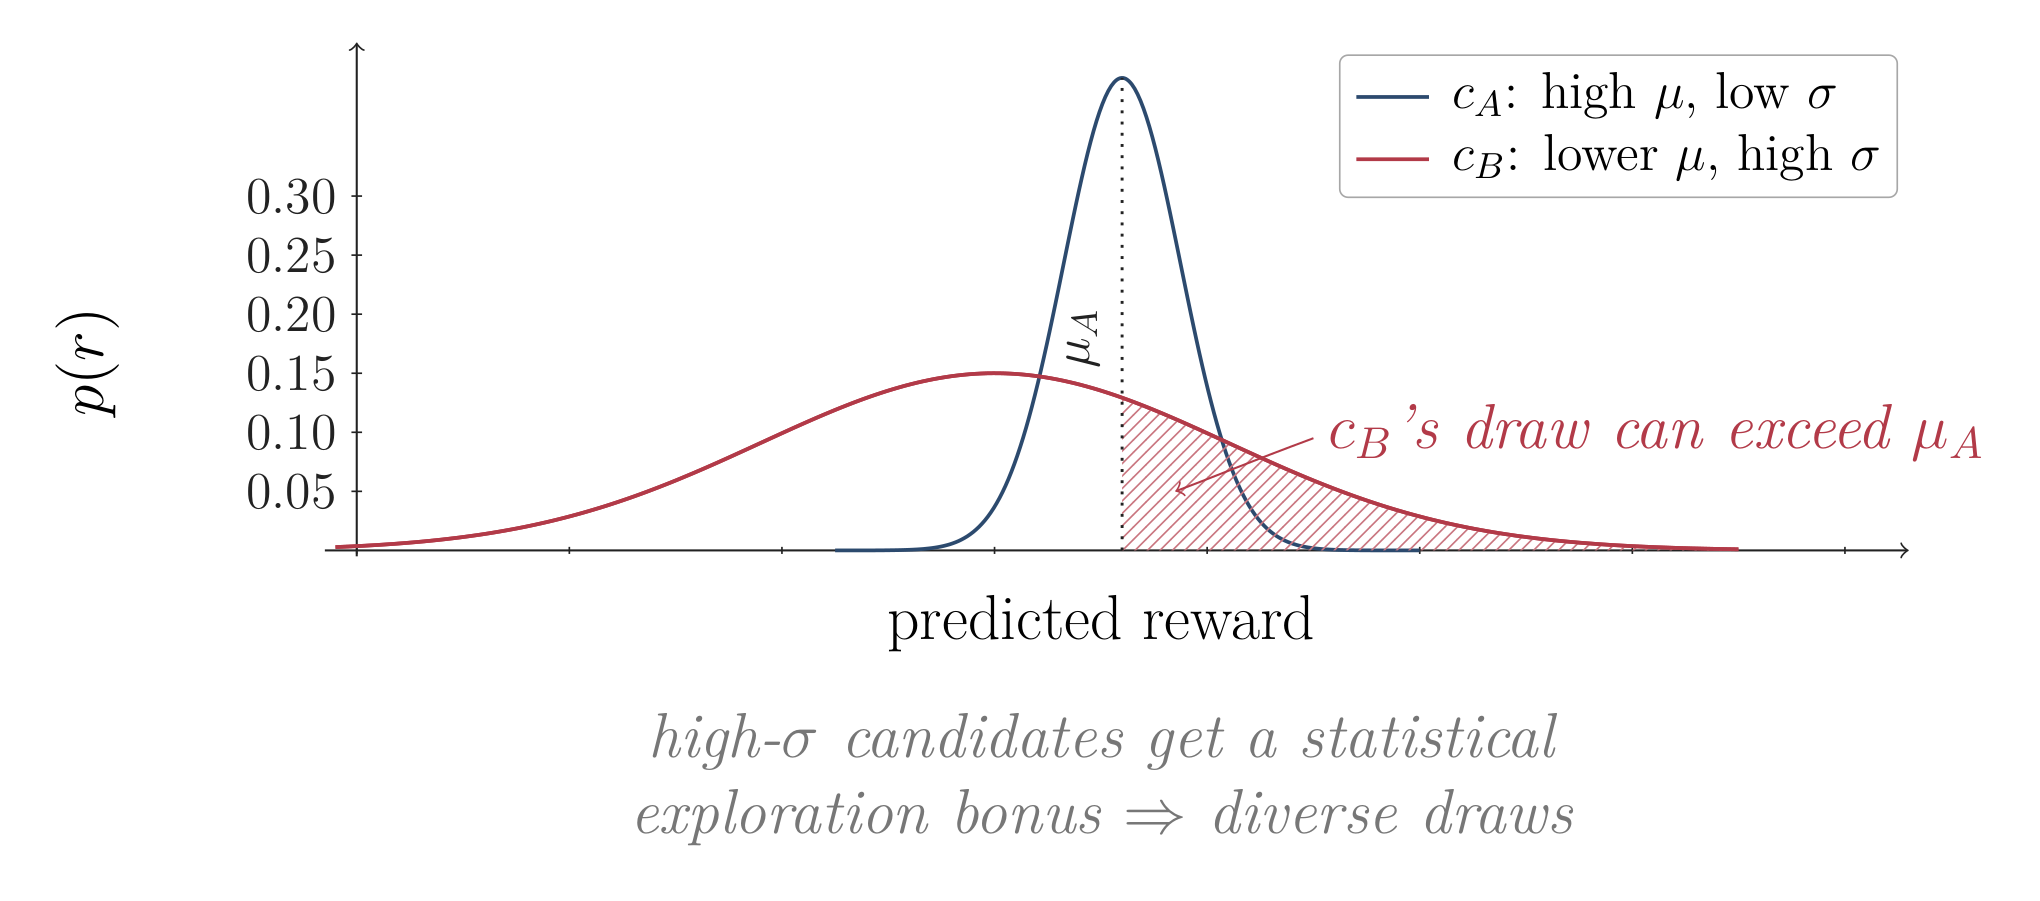
\includegraphics[width=0.65\textwidth]{figures/diagram_thompson.png}
  %\vspace{-0.15in}
  %\caption{\textbf{Thompson sampling.} Two candidates' %ensemble posteriors over predicted reward: $c_A$ (low %$\sigma$, greedy pick at $\mu_A$) and $c_B$ (lower mean, higher $\sigma$). Hatched area $= \Pr[\hat r_B > \mu_A]$ is the probability that $c_B$'s Thompson draw exceeds the deterministic-greedy threshold.}
  %\label{fig:diag_thompson_body}
%\end{figure}
\begin{figure}[b]
  \centering
  \begin{minipage}[t]{0.64\textwidth}
    \vspace{0pt}
    \centering
    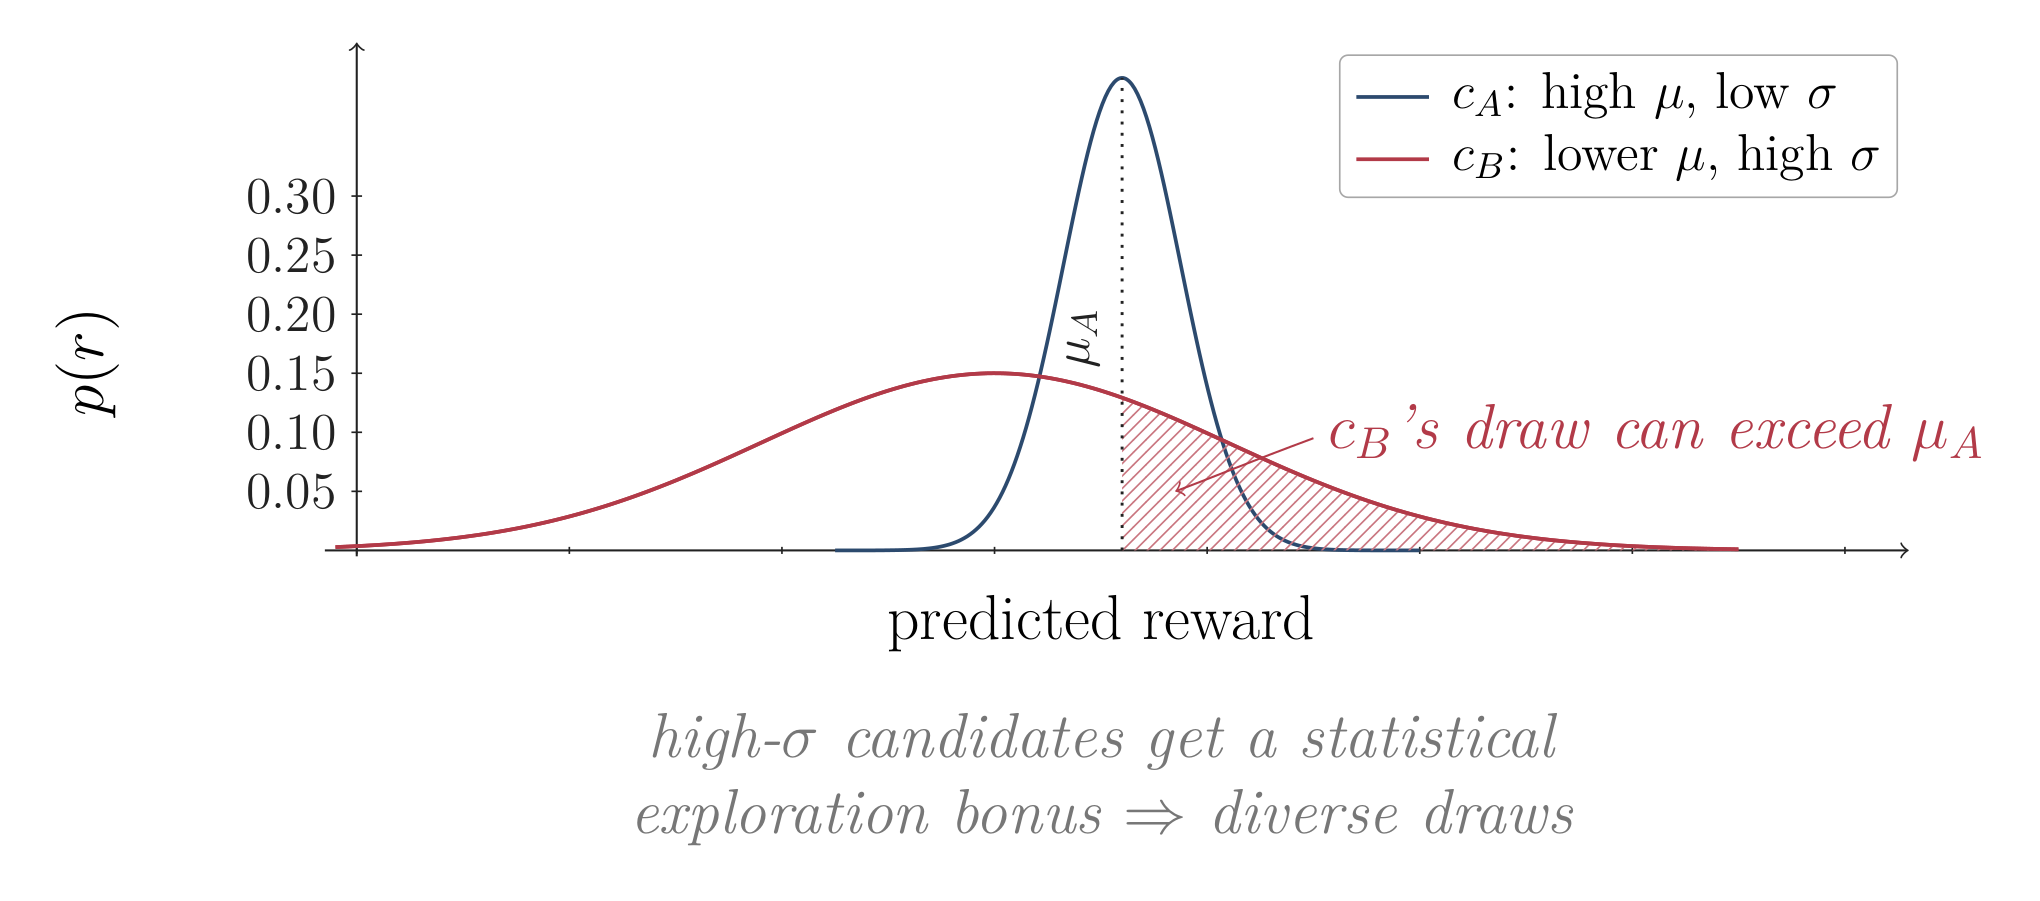
\includegraphics[width=\linewidth]{figures/diagram_thompson.png}
  \end{minipage}
  \hfill
  \begin{minipage}[t]{0.35\textwidth}
    \vspace{0pt}
    \caption{\textbf{Thompson sampling.} Although $c_A$ has the higher mean prediction, $c_B$ can be selected because its larger uncertainty gives it nonzero probability of drawing above the greedy threshold.}
    \label{fig:diag_thompson_body}
  \end{minipage}
\end{figure}


\textbf{Thompson Sampling Acquisition.} Because the oracle budget is finite, the loop must choose a small subset of generated candidates for evaluation. The simplest rule evaluates the candidates with the highest predicted reward under a surrogate model. This greedy rule is purely exploitative: it spends oracle calls where the surrogate already predicts high reward. We also consider uncertainty-aware acquisition using Thompson sampling \citep{thompson1933likelihood, russo2018tutorial}. Given an ensemble surrogate with mean $\mu_i$ and disagreement $\sigma_i$ for candidate $x_i\in C_t$, Thompson sampling draws a sampled reward estimate:
\[
\hat r_i = \mu_i + \varepsilon_i \sigma_i, \qquad \varepsilon_i \sim \mathcal{N}(0,1),
\]
and evaluates the top-$K$ candidates by $\hat r_i$, defining the selected batch $S_t$. Fig.~\ref{fig:diag_thompson_body} depicts the intuition behind how Thompson sampling balances the explore/exploit trade-off.  Candidates with high uncertainty can outrank candidates with higher predicted mean but lower uncertainty, i.e., this scheme incentivizes to explore seemingly lower quality but high uncertainty candidates. %This uses oracle calls to reduce uncertainty in promising regions rather than only confirming the surrogate's current maximum.


% The contrast with deterministic top-$\mu$ selection is sharp (Fig.~\ref{fig:diag_thompson_body}): under deterministic selection a candidate $c_B$ with $\mu_B < \mu_A$ never gets oracle-evaluated, no matter how uncertain it is, so the training data $(x, r(x))$ that downstream finetuning sees is concentrated on the current surrogate argmax. As the ensemble disagreement $\sigma_B$ grows away from zero, the Thompson rule smoothly transitions from this hard-greedy regime to a stochastic exploration bonus, the standard way to guard against local optima \citep{chapelle2011empirical}. The acquisition step is itself modifying which samples from $p_{\theta_t}$ enter the evaluated set and therefore which data the gradient computes against. A fuller comparison against deterministic top-$\mu$ selection is given in Appendix~\ref{app:knob-interactions}.




%\begin{figure}[t]
%  \centering
%  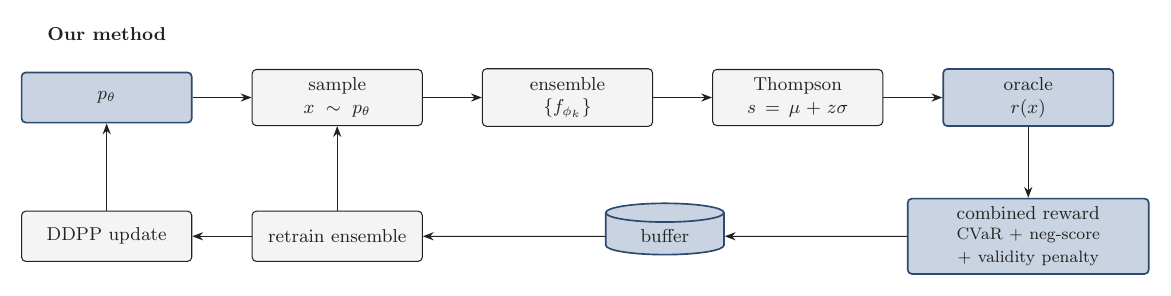
\includegraphics[width=0.95\textwidth]{figures/diagram_final.png}
%  \caption{\textbf{Online active loop.} Schematic of the composable-knob harness evaluated in this paper. Each round samples $M$ candidates from $p_{\theta_t}$, scores them under the surrogate ensemble, oracle-evaluates the Thompson-selected top-$K$ (with invalid candidates assigned $r_{\text{inv}}$ before they reach the oracle), pushes the resulting $(x, r)$ pairs to the buffer, and updates $p_{\theta_t}$ to $p_{\theta_{t+1}}$ via DDPP-LB on the CVaR + debiasing-shaped log-reward; the ensemble is refit on the buffer at the end of each round. Pseudocode in Appendix~\ref{app:diagrams}, Algorithm~\ref{alg:method}.}
%  \label{fig:diag_final}
%\end{figure}

\subsection{Adaptation Strategies}\label{sec:adaptation_design}

\textbf{CVaR-Style Reward Shaping.}
\looseness -1 A second lever acts on the reward itself after oracle evaluation and before it enters the gradient. We write the resulting shaped training reward as $\tilde r(x)$. Because the design objective in Eq. \eqref{eq:design_objective} is controlled by the upper tail rather than the average generated molecule, we adapt the model via a CVaR-style \citep{rockafellar2000cvar, rockafellar2002cvar} objective (Fig.~\ref{fig:diag_reward_shaping}(a)), as introduced in prior work on diffusion model adaptation~\citep{santiFlowDensityControl, wang2026efficient}. This objective allows to sacrifice the average sample reward to enhance the quality of top-samples:
\[
\mathrm{CVaR}_{1-\tau}[r(x)]
=
\mathbb{E}\!\left[
r(x) \mid r(x) \ge Q_\tau(r)
\right].
\]
% Upper-tail shaping alone can still repeatedly reinforce regions the generator already samples frequently, so we add a score-based debiasing term:
% \[
% \log \tilde r_{\mathrm{debias}}(x)
% =
% \log \tilde r_{\mathrm{cvar}}(x) - \gamma \log p_{\theta_t}(x),
% \]
% where $\log p_{\theta_t}(x)$ denotes the model likelihood term used inside the discrete diffusion training dynamics. At the loop level, $x$ is a candidate molecule; inside the denoising loss, the same notation may refer to the corresponding noised or partially denoised state. The value is treated as a constant for gradient purposes. This favors candidates that are high reward but not already high likelihood under the current generator.

\begin{figure}[htbp]
  \centering
  \begin{minipage}[c]{0.49\textwidth}\centering
    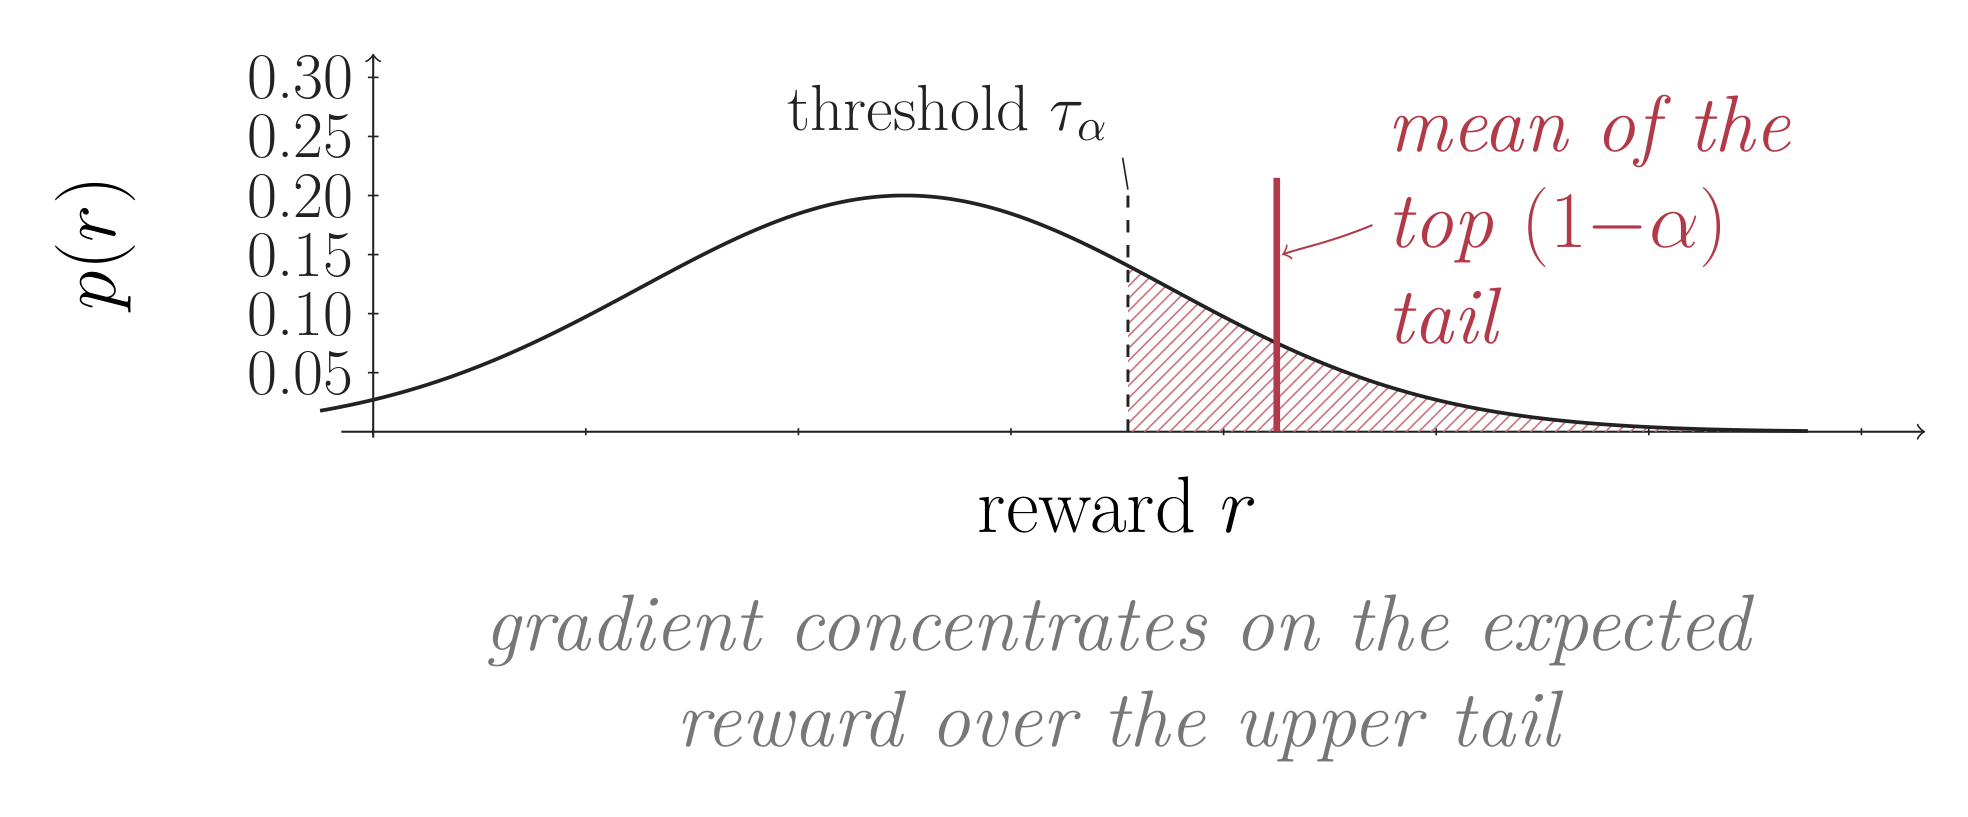
\includegraphics[width=\textwidth]{figures/diagram_cvar.png}\\
    \textbf{(a)} CVaR Shaping
  \end{minipage}\hfill
  \begin{minipage}[c]{0.49\textwidth}\centering
    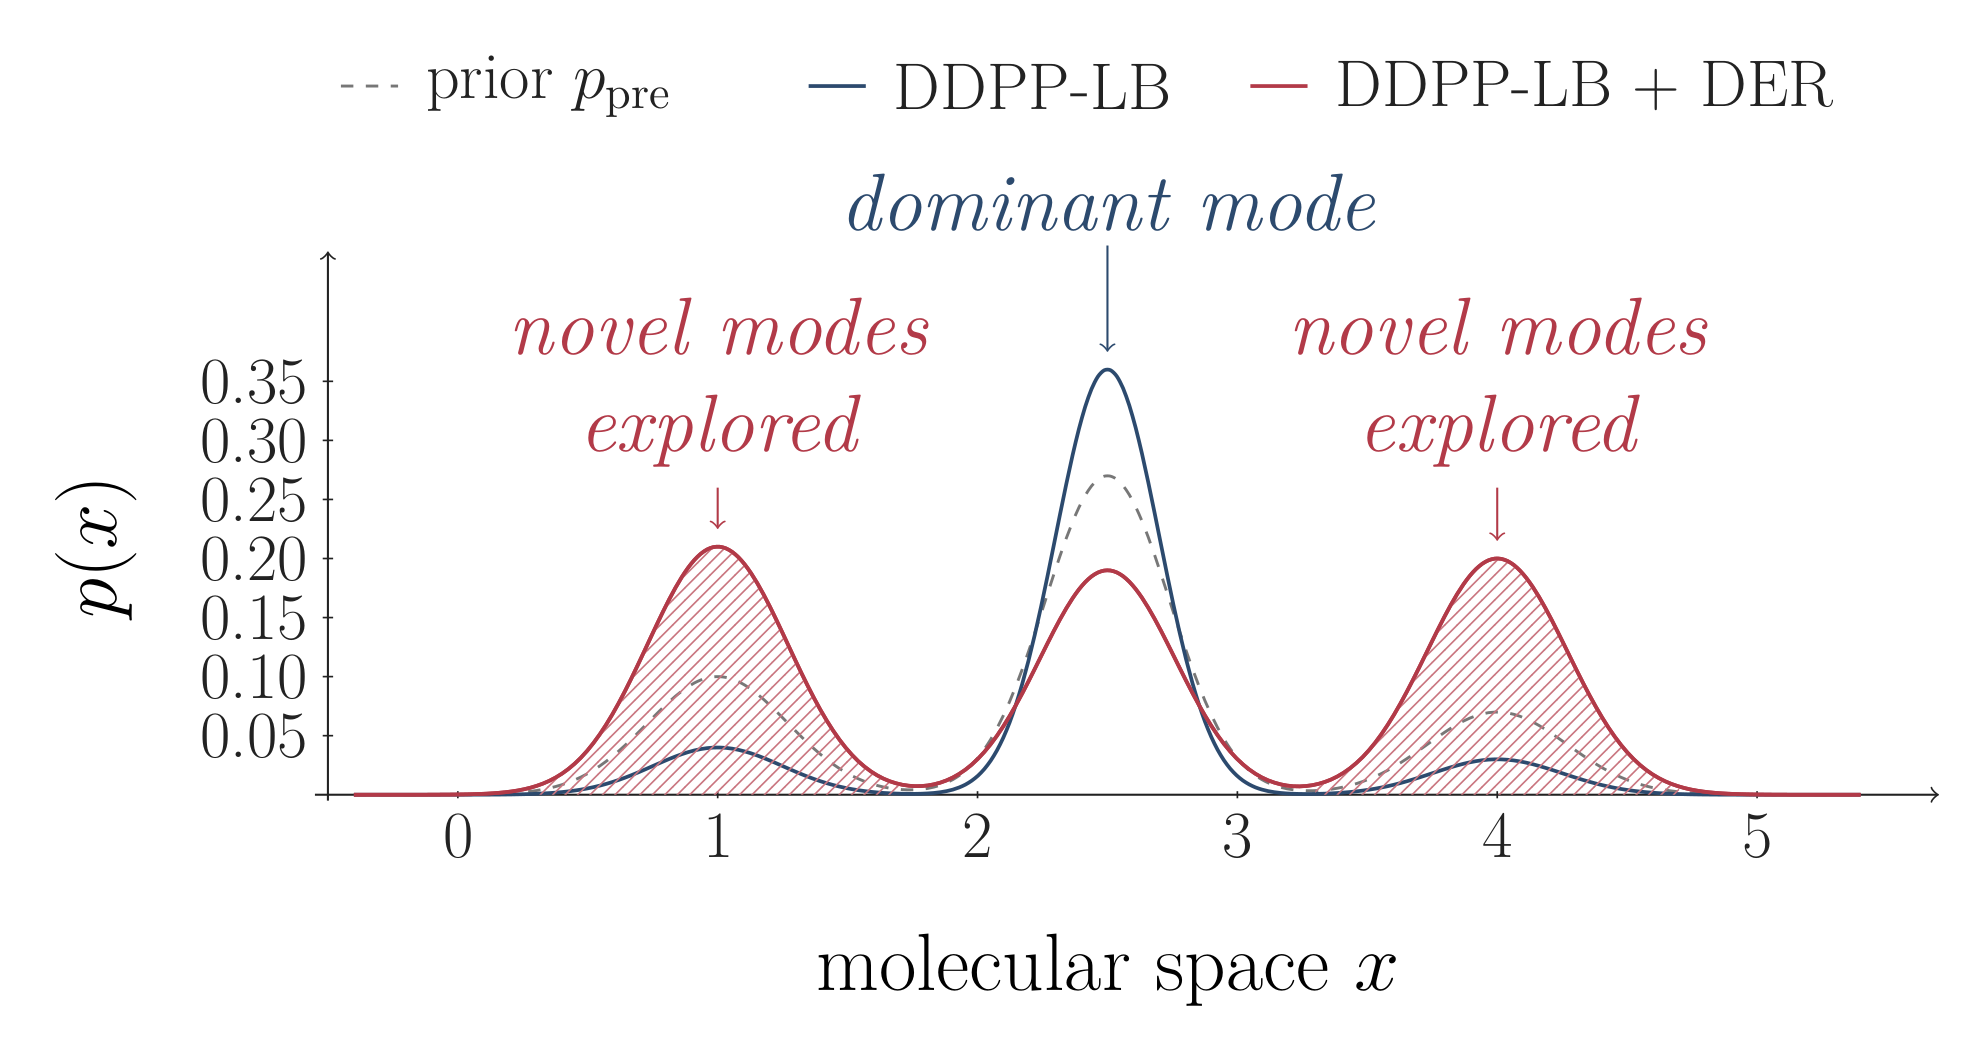
\includegraphics[width=\textwidth]{figures/diagram_debiasing.png}\\
    \textbf{(b)} Density Entropy Regularization
  \end{minipage}
  \caption{\textbf{Reward-shaping and model debiasing} \textbf{(a)} CVaR upper-tail shaping: the right-tail of the reward distribution above the $\tau$-quantile (dashed) is shaded, and the solid red bar marks $\mathrm{CVaR}_{1-\tau} = \mathbb{E}[r \mid r \geq Q_\tau]$, the expected reward conditional on being in that tail. Optimization concentrates gradient on this tail expectation, not on a hard top-$k$ selection. \textbf{(b)} Density Entropy Regularization (model debiasing): subtracting the current generator's diffusion-internal likelihood $\log p_{\theta_t}(x)$ from the log-reward redistributes gradient mass off densely-occupied modes and toward less-frequented regions, exposing minor modes the unshaped reward would have kept under-explored.}
  \label{fig:diag_reward_shaping}
  \label{fig:diag_cvar_body}
  \label{fig:diag_debiasing_body}
\end{figure}

\textbf{Density Entropy Regularization.}
CVaR reward shaping focuses the update on the upper tail, but it does not distinguish between high-reward regions that the generator already samples frequently and high-reward regions that remain underexplored. To expose this distinction independently of CVaR, practitioners can apply a density-entropy regularizer~\citep{de2025provable, santiFlowDensityControl, santiVerifierConstrainedFlowExpansion2026} that uses the current model density as a measure of how occupied a region is under the generator and shapes the raw log-reward as:
\begin{equation}
\log \tilde r_{\mathrm{debias}}(x)
=
\log r(x) - \gamma \log p_{\theta_t}(x),
\label{eq:debias}
\end{equation}
illustrated in Fig.~\ref{fig:diag_reward_shaping}(b), where $\log p_{\theta_t}(x)$ is the marginal. In continuous-diffusion analyses~\citep{de2025provable, santiFlowDensityControl}, the corresponding negative-score gradient $\nabla_x \log p_{\theta_t}(x)$ can be directly approximated by the available score network,  but in masked discrete diffusion it is estimated by the marginalization:
\[
p_{\theta_t}(x_0) \;=\; \mathbb{E}_{t, \, x_t \sim q(x_t \mid x_0)}\!\bigl[\,p_{\theta_t}(x_0 \mid x_t)\,\bigr] \cdot \text{(noise-schedule weight)},
\]
a sum over an exponentially-large set of noised states $x_t$, making it intractable. For discrete diffusion the proper asymptotic unbiased estimator is a Monte-Carlo ELBO \citep{nie2025llada} (LLaDA, Algorithm~3), which costs $n_{\text{mc}}$ extra forward passes per evaluation.

We replace $\log p_{\theta_t}(x)$ in Eq.~\ref{eq:debias} with the cheapest such estimator: 
\[
\widehat{\log p_{\theta_t}(x)} \;\equiv\; \log p_{\theta_t}(x_0 \mid x_t)
\;=\;
\textstyle\sum_{i \,:\, x_t^i = [\text{MASK}]}\, \log \mathrm{softmax}(\ell_i)\bigl[x_0^i\bigr].
\]
This estimator is a cheap approximation of the diffusion ELBO, so it is not equivalent to the MCMC-estimated continuous negative-score regularizer or to the LLaDA-style $L/l$-weighted estimator in the limit. We choose this estimator  for computational reasons: the alternatives cost $n_{\text{mc}}\!\times$ extra forward passes per gradient step, which is prohibitive across thousands of online finetuning steps. Despite the approximation, we find empirically that it induces the intended distribution shift and that the added noise leads to more exploration and overall better performance. we find empirically that it achieves comparable oracle-call efficiency to LLaDA-Alg.\,3 variants with $n_{\text{mc}} \in \{1, 4, 8, 16\}$ while being substantially faster per GPU hour. Post-hoc evaluation with the unbiased LLaDA-Alg.\,3 estimator ($n_{\text{mc}}{=}32$) confirms that the resulting NLL distributions from the cheap estimator follows closely to the LLaDA estimator with wider exploration (Appendix Figs.~\ref{fig:negscore_estimator_curves} and~\ref{fig:negscore_nll_dist}).
Intuitively, this term favors candidates that are high reward but not already high likelihood under the generator, complementing Thompson-sampling acquisition (acquisition vs.\ reward-shape act on the loop at different points; see Appendix~\ref{app:knob-interactions} and Fig.~\ref{fig:diag_debiasing_body}).
The estimated value is detached, so the parameter gradient enters the standard DDPP-LB / VIDD policy-gradient term as a scalar reward modifier  (Appendix~\ref{app:method-details}).


\subsection{Objective-mismatch corrections}\label{sec:design-objmismatch}

Once exploration starts shifting $p_{\theta_t}$ off the prior's dominant modes, two gaps open between what the gradient actually optimizes and the true objective. The next two components can close them.

\textbf{Replay Buffer.}
A remaining choice is which evaluated samples appear in each update. A purely on-policy update trains only on the latest batch, so useful molecules discovered early stop influencing the generator once the sampling distribution moves on. We therefore optionally train from a replay buffer that mixes fresh candidates with retained high-reward samples \citep{mnih2015human, schaul2016prioritized, olivecronaMolecularNovoDesign2017}. Concretely, the buffer is fixed-capacity FIFO with priority eviction (when full, the lowest-reward sample leaves first, not the oldest), and each minibatch is drawn by stratified sampling across reward bins so high-reward outliers don't get diluted by a larger volume of mid-reward fresh candidates.

\textbf{Invalid-output penalty.}
To keep optimization on the molecular manifold, candidates that fail validity checks, ie RDKit parsing \citep{rdkit} in the case of small molecules, receive a fixed penalty $r_{\mathrm{inv}}<0$ and enter training as low-reward examples. The mismatch this corrects is between the oracle's reward (defined for any string) and the actual objective (high reward on a valid molecule); the penalty closes that gap by giving the gradient an explicit signal to pull $p_{\theta_t}$ back toward the valid molecular manifold.